\documentclass[12pt]{article}

\usepackage[T1,T2A]{fontenc}
\usepackage[utf8]{inputenc}
\usepackage[bulgarian]{babel}
\usepackage{graphicx}
\usepackage{amssymb}
\usepackage{amsmath}
\usepackage{commath}
\usepackage{float}
\usepackage{booktabs}   
\usepackage{ltablex}

\parindent 0px % turn off indenting

% have nicer-looking links
\usepackage{hyperref}
\hypersetup{
  colorlinks   = true, %Colours links instead of ugly boxes
  urlcolor     = red, %Colour for external hyperlinks
  linkcolor    = blue, %Colour of internal links
  citecolor   = blue
}
\usepackage[hypcap=true]{caption}


\newcommand{\JMUTitle}[9]{

  \thispagestyle{empty}
  \vspace*{\stretch{1}}
  {\parindent0cm
  \rule{\linewidth}{.7ex}}
  \begin{flushright}
    \vspace*{\stretch{1}}
    \sffamily\bfseries\Huge
    #1\\
    \vspace*{\stretch{1}}
    \sffamily\bfseries\large
    #2\\
    \vspace*{\stretch{1}}
    \sffamily\bfseries\small
    #3
  \end{flushright}
  \rule{\linewidth}{.7ex}

  \vspace*{\stretch{1}}
  \begin{center}
    
\includegraphics[width=3in]{./images/logo.png} \\
    \vspace*{\stretch{1}}
    \Large Курсов проект по \\ \textit{Извличане на информация} \\

    \vspace*{\stretch{2}}
    \large Факултет по математика и информатика\\
    \large Софийски университет\\
    
    \vspace*{\stretch{1}}
    \large Лектор: #8 \\[1mm]
    
    \vspace*{\stretch{1}}
    \large #7 \\

  \end{center}
}

\newcommand*{\MyIndent}{\hspace*{7em}}

%%%%%%%%%%%%%%%%% END OF PREAMBLE %%%%%%%%%%%%%%%%



\begin{document}  

  \JMUTitle
      {Ati: Система за разпознаване на авторство}
      {Симеон Христов}
      {6MI3400191}
      
      {Wirtschaftswissenschaftlichen Fakultät}  % Name der Fakultaet
      {W"urzburg 2018}                          % Ort und Jahr der Erstellung
      {Февруари 2023}                              % Tag der Abgabe
      {проф. Иван Койчев}               % Name des Erstgutachters
      {Zweitgutachter}                          % Name des Zweitgutachters

  \clearpage

\tableofcontents

\clearpage

\section{Увод}

    Целта на проекта е създаването на категоризационна система, която при даден корпус от документи - $D$, всеки от които е написан от един автор $y$, да идентифицира автора на анонимен текст $x$.
    
    \vspace{1em}
    
    Разработената система може да бъде основата за разработване на приложение, което да:
    
    \begin{enumerate}
        \item \textbf{Проверява на авторство}: Дали даден текст наистина е написан от определен автор?
        \item \textbf{Открива плагиатство}: Намиране на прилики между два или повече текста;
        \item \textbf{Създава профил или характеризира на даден автора}: Извличане на информация за възрастта, образованието, пола и т.н. на автора на даден текст;
        \item \textbf{Открива стилистични несъответствия} (както може да се случи при съвместно писане): Дали авторът настина е само един?
        \item \textbf{Отговоря на въпроси}: В матурата по български език и литература има въпроси, които са фокусирани върху разпознаване на автора на даден отказ или разпознаване на автора, който пише за определен герой.
    \end{enumerate}
    
    \vspace{1em}
    
    Задачите, които са реализирани от този проект са:
    
    \begin{enumerate}
        \item Създаване на паяк, копаещ документи (текстовете на съответните автори) от уеб страница.
        \item Създаване на модел, който е трениран върху тренировъчно множество ($80\%$ от данните), валидиран върху валидационно множество ($10\%$ от оставащи данни) и оценен върху тестово множество (последните $10\%$ оставащи данни).
        \item Сравняване на поне 3 стилистични метрики за всички автори.
        \item Сравняване на различни представяния на текст: \textit{tf-tdf} и \textit{transformer sentence embeddings}.
        \item Сравняване на класификатори: един и ансамбъл.
        \item Създаване на потребителски интерфейс.
    \end{enumerate}
    

\section{Преглед на областта по разпознаване на авторство}

[ ] TODO: Подходи и методи за решаване; съществуващи решения; сравнителен анализ на решенията./ Подобни изследвания.


\section{Проектиране}

    От гледна точка на машинното самообучение системата е представена схематично на \hyperref[fig:bigP]{Фигура~\ref*{fig:bigP}}.
    
    \begin{figure}
    \centering
        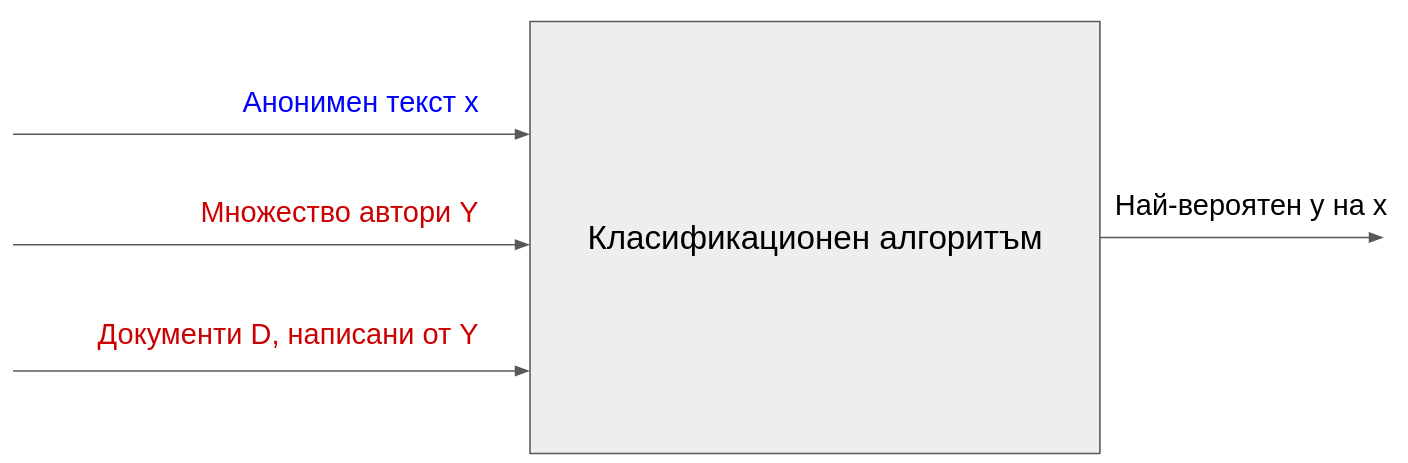
\includegraphics[scale=0.3]{./images/big_picture.png}
        \caption{Системата, представена "от птичи поглед".}
        \label{fig:bigP}
    \end{figure}
    
    Потребителският интерфейс е представен на .
    
    
    [ ] TODO: Анализ на изискванията, Обща архитектура – напр. слоеве, модули, блокове, компоненти...; Модел на данните; Схема за представяне на знанията. Диаграми; Потребителски интерфейс (ако има); Ресурсни;…
    
\section{Реализация, тестване/експерименти}

\subsection{Използвани технологии, платформи и библиотеки}

[ ] TODO: Подходящи средства за реализация за проекта (технологии, платформи и библиотеки). Избор на средствата и начин за използването им;

\subsection{Реализация/Провеждане на експерименти}

[ ] TODO: Реализация (на модулите); 
За система/приложение: На кратко: планиране на тестването - тестови сценарии,...; Анализ на резултатите.

\section{Заключение}

[ ] TODO: Обобщение на направеното/резултатите. 
Идеи за по-нататъшно развитие, усъвършенстване или други експерименти.

\section{Използвани технологии}

[ ] TODO: (статии, книги, онлайн ресурси, форматирани съгласно MLA Style - http://www.library.mun.ca/guides/howto/mla.php) или друг подобен стандарт.

%%%%%%%%%%%%%%%%% END OF MAIN TEXT %%%%%%%%%%%%%%%%

\section{Използвана литература}

% Has to be formatted using MLA style.

\listoffigures

\end{document}